\documentclass[12pt,a4paper]{article} % din a4, 11 pt schrift, einseitig,
\usepackage{graphicx} % Allows including images
\usepackage{float}
\usepackage{amsmath}
\usepackage{amsfonts,amssymb,amsbsy,latexsym,amsmath,tabulary,graphicx,times,caption,fancyhdr}
\begin{document}
\section{Product List by Category}
\BLOCK{ for key, value in names | dictsort}
\subsection{Category \VAR{key}}
\begin{tabular}[!ht]{ll}
    Index & Name \\
    \hline
    \BLOCK{ for inner_key, inner_value in value | dictsort}
        \VAR{inner_key}& \VAR{inner_value['Name']}\\
    \BLOCK{ endfor }
\end{tabular}
\BLOCK{ endfor }\\
\\ \\
{\noindent \textbf{As you can see the tables/graphs are automatically generated . After editing this tex file in a way you like it and only for once, you can have this report automatically for any other new data}}.\\
\begin{figure}[!ht]
	\centering
	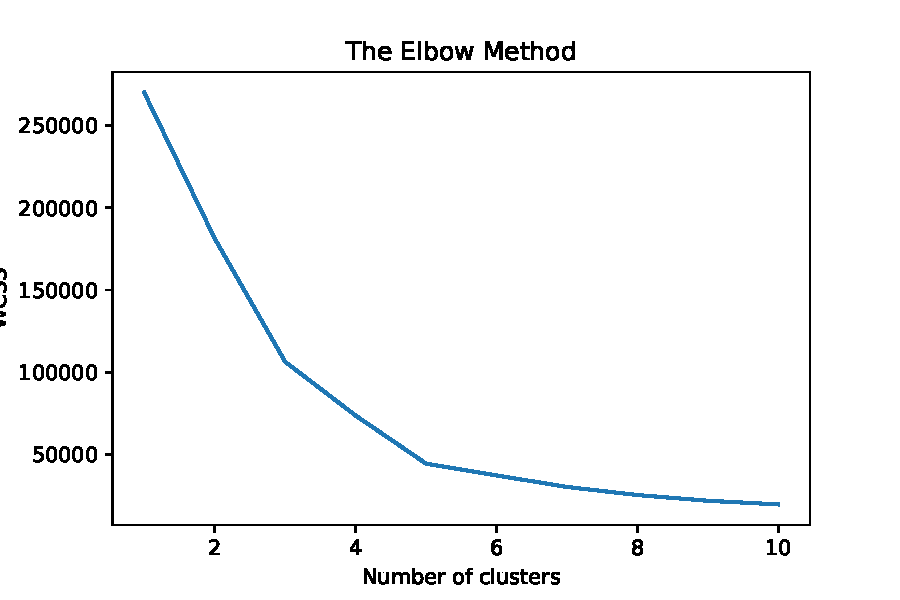
\includegraphics[width=12cm]{figure_1.pdf}
	\caption{Figure 1}
\end{figure} \\
\begin{figure}[!ht]
	\centering
	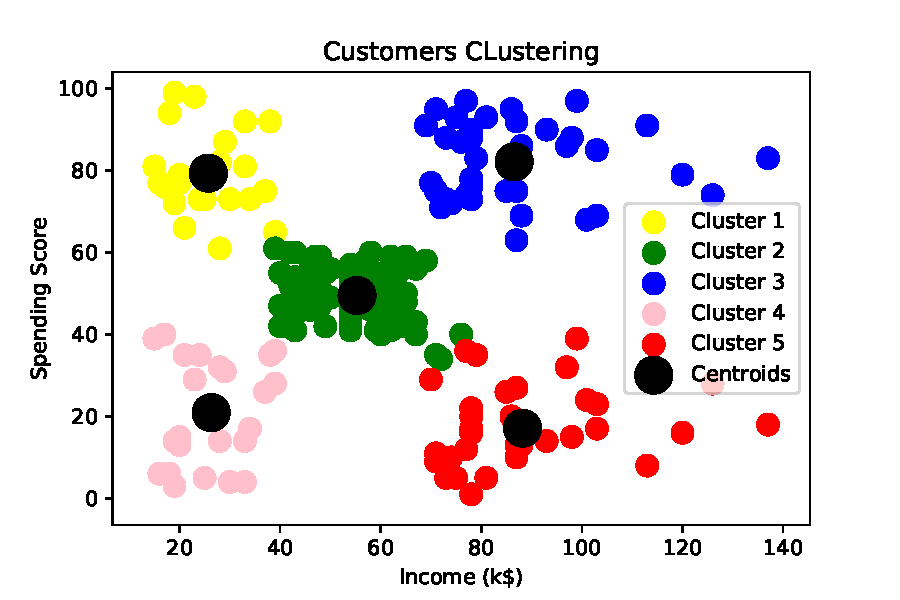
\includegraphics[width=12cm]{figure_2.pdf}
	\caption{Figure 2:}
\end{figure} 

\end{document}
